\section{$n$阶展开方法}
\begin{frame}{$n$阶展开方法}
齐次平衡原则是很多算法的基础, 如双曲正切方法, Painleve展开方法, Jacobi椭圆函数方法等. 我们以双曲正切方法为例来展示$n$解展开方法对齐次平衡原则的改进. 
\end{frame}



\begin{frame}{$n$阶展开方法解双曲正切函数解}
\begin{enumerate}
\item 双曲正切方法
\item 三类平衡点
\item $n$阶展开多项式的性质
\item 例1: (4+1)Fokas 方程三类平衡点都有
\item 例2: (1+1)EMM 方程第三类平衡点的决定性作用 
\item 例3: 上界的作用
\end{enumerate}
\end{frame}

\begin{frame}{双曲正切方法}
考虑非线性演化方程 
\[
    U\sbrace{u,u\up{1},u\up{2},\cdots}=0, 
\]
其中$u=u(x_1,\cdots,x_d)$, 而$u\up{k}$表示$u$的所有$k$阶导数的集合, 例如$u\up{1}=\bbrace{u_{x_1},\cdots,u_{x_d}}$. 
将
\[
    u=\sum_{k=0}^{m}{a_k\tanh^k(\xi)}
\]
代入原方程后, 方程中各个加法项都是关于$\tanh(\xi)$的多项式, 设他们的次数为 
\[
    s_1 m+d_1,\cdots,s_l m + d_l . 
\]
\end{frame}

\begin{frame}{三类平衡点}
在齐次平衡原则中, 以往通过
\[
    s_i m+d_i=s_j m+d_j, s_i\neq s_j , m\in \mathbb Z_+. 
\]
来确定$m$的值, 没有考虑$s_i=s_j$的情况. 但是我们不能否定该情况下平衡的可能性, 所以我们重新定义平衡的条件如下:
\begin{itemize}
    \item 整数性: $ m\in \mathbb Z_+$ 
    \item 平衡性: $\exists i\neq j, s_i m+d_i=s_j m+d_j $
    \item 最大性: $\forall k \not\in \bbrace{i,j}, s_i m+d_i\ge s_k m+d_k $
\end{itemize}
\end{frame}

\begin{frame}
\begin{columns}
\begin{column}{.5\textwidth}
\begin{figure}
\centering
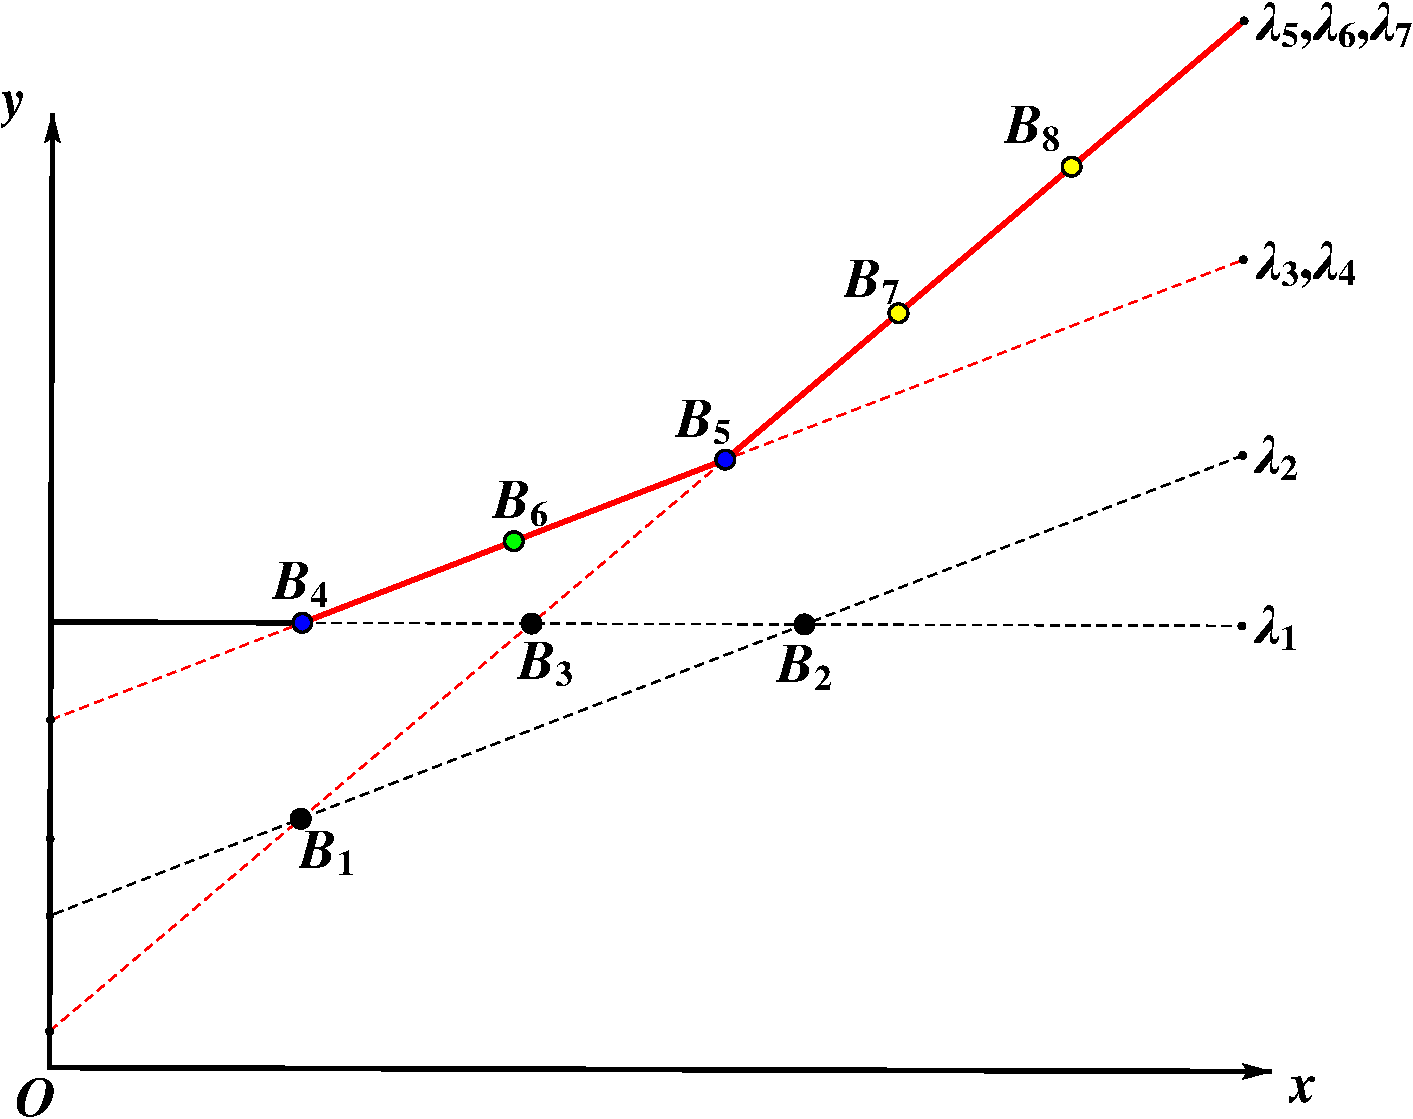
\includegraphics[width=\textwidth]{../paper/fig/ps.pdf}
\caption{平衡点分类示意图}
\end{figure}
\end{column}
\begin{column}{.5\textwidth}
\[
    \lambda_k = s_k m + d_k 
\]
\begin{itemize}
\item $B_1,B_2,B_3$不满足最大性条件, 不是平衡点. 
\item $B_4,B_5$可以由平衡性条件唯一确定, 是\textbf{第一类平衡点}. 
\item $B_6$不能由平衡性条件唯一确定, 但是可以由最大性条件确定, 是\textbf{第二类平衡点}.
\item $B_7,B_8$以及右侧的一系列整点, 满足三种平衡条件, 但无法确定其上界, 是\textbf{第三类平衡点}. 所以我们提出了$n$阶展开方法来确定此类平衡点的上界. 
\end{itemize}
\end{column}
\end{columns}
\end{frame}

\begin{frame}{$n$阶展开方法}
\small
因为求导会使得$m$出现在系数中, 所以我们可以通过方程最高$n$项的系数来分析$m$的上界, 所以我们提出了$n$阶展开方法. 

考虑一个关于$x$的$m$次多项式, 其$n$阶展开形式为
\[
    F\sbrace{x,m,u\up n}=\sum_{k=0}^{n-1}{u_k x^{m-k}}+\OO\sbrace{x^{m-n}},
\]
其中 
\[
\OO\sbrace{x^n}=\left\{
\begin{array}{cl}
\text{次数不超过}\,n\,\text{的多项式} & n\ge 0, \\
0                                    & n<0 .
\end{array}
\right.
\]
在双曲正切方法中, 取
\[
    u=F\sbrace{\tanh(\xi),m,a\up{n}}=\sum_{k=0}^{n-1}{a_k \tanh^{m-k}(\xi)}+\OO(\tanh^{m-n}(\xi))
\]
代入原方程, 将方程转化为关于$\tanh(\xi)$的$n$阶展开多项式, 所以我们要考虑$n$阶展开多项式的乘法, 求导和加法的规则. 
\end{frame}

% \begin{frame}{$n$阶展开多项式的性质}
% \begin{itemize}
% \item $n$阶展开多项式的相乘还是$n$阶展开多项式.
% \item $n$阶展开多项式求导后, 其系数中将会包含$m$.
% \item $n$阶展开多项式加法的约束条件.
% \end{itemize}
% \end{frame}

\begin{frame}{$n$阶展开多项式的乘法}
\[
\begin{aligned}
& F\sbrace{x,m,u \up n}\cdot F\sbrace{x,l,v\up n} \\
=& \mbrace{\sum_{k=0}^{n-1}{u_k x^{m-k}}+\OO\sbrace{x^{m-n}}}\mbrace{\sum_{k=0}^{n-1}{v_k x^{l-k}}+\OO\sbrace{x^{l-n}}} \\
=& \mbrace{\sum_{k=0}^{n-1}{u_k x^{m-k}}}\mbrace{\sum_{k=0}^{n-1}{v_k x^{l-k}}}+\OO\sbrace{x^{m+l-n}} \\
=& \sum_{p=0}^{n-1}{x^{m+l-p}\mbrace{\sum_{k=0}^p{u_k v_{p-k}}}}+\OO\sbrace{x^{m+l-n}} \\
=& F\sbrace{x,m+l,w\up n} 
\end{aligned} 
\]
\end{frame}

\begin{frame}{$n$阶展开多项式的求导}
\[
\begin{aligned}
& \DIF{t}F\sbrace{x,m,u\up{n}}  \\
=& \DIF{t}\sbrace{\sum_{k=0}^{n-1}{u_k x^{m-k}}+\OO(x^{m-n})} \\
=& \sum_{k=0}^{n-1}{\DIFF{u_k}{t}x^{m-k}}+\DIFF{x}{t}\cdot\sum_{k=0}^{n-1}{u_k (m-k) x^{m-k-1}}+\DIFF{x}{t}\cdot\OO(x^{m-n-1}) \\
=& \sum_{k=0}^{n-1}{\DIFF{u_k}{t}x^{m-k}}+\DIFF{x}{t}\cdot\sbrace{\sum_{k=0}^{n-1}{u_k (m-k) x^{(m-1)-k}}+\OO\sbrace{x^{(m-1)-n)}}} \\ 
=& F\sbrace{x,m,v\up{n}}+\DIFF{x}{t}\cdot F\sbrace{x,m-1,w\up{n}} 
\end{aligned}
\]
\end{frame}


\begin{frame}{$n$阶展开多项式的加法}
考虑加法 
\[
    F\sbrace{x,s_i m+d_i,u\up n}+F\sbrace{x,s_j m+d_j,v\up n}
\]  
因为我们无法比较$s_i m + d_i$ 和 $s_j m + d_j$ 大小, 所以无法直接求和. 

假设$F\sbrace{x,s_j m+d_j,v\up n}$在求和时不会影响$F\sbrace{x,s_i m+d_i,u\up n}$的前$n$项, 则需 
\[
    s_i m+d_i - n > s_j m+d_j 
\]
从而 
\[
\begin{aligned}
&F\sbrace{x,s_i m+d_i,u\up n}+F\sbrace{x,s_j m+d_j,v\up n} \\
=&\left\{
\begin{array}{cl}
    F\sbrace{x,s_i m+d_i,u\up n} & s_i>s_j,            \\
    F\sbrace{x,s_i m+d_i,w\up n} & s_i=s_j.
\end{array}
\right.
\end{aligned}
\]
\end{frame}

\begin{frame}{确定第三类平衡点的上界}    
\small 
将$F\sbrace{\tanh(\xi),m,a\up{n}}$代入原方程, 则原方程的$n$阶展开形式为
\[
    F\sbrace{\tanh(\xi),\sigma m+\delta,\Omega\up{n}}=0 .
\]
设$\Omega_{k}$是第一个非零项的系数, 则: 

(一) $\Omega_{k}=0$关于$m$有正整数解, 此时$m$的上界为
\[
    m_{31}=\max\bbrace{m\in \mathbb Z_+|\Omega_{k}=0}.
\]

(二) $\Omega_{k}=0$关于$m$没有正整数解, 这说明若加法的假设条件成立, 则原方程无解. 所以需要加法的假设条件不成立才可能有解, 此时需要满足 
\[
    \forall s_j<\sigma, \sigma m + \delta - k \le s_j m + d_j
\]
则有
\[
    m\le m_{32} = \underset{s_j<\sigma}{\max}{\frac{d_j-\delta+k}{\sigma-s_j}}
\]
最终, 第三类平衡点的上界为 
\[
    m_3 = \max\bbrace{m_{31},m_{32}}. 
\]
\end{frame}

\begin{frame}{示例}
下面我们通过三个实例来说明$n$阶展开方法的思路和步骤. 

\end{frame}

\begin{frame}{例1: (4+1)Fokas方程(含全部三类平衡点)}
% \small 
\begin{equation*}
    u_{tx}-\frac{1}{4}u_{xxxy}+\frac{1}{4}u_{xyyy}+3u_xu_y+3uu_{xy}-\frac{3}{2}u_{wz}=0 ,
\end{equation*}
其阶数列表为$\mbrace{m+2,m+4,m+4,2m+2,2m+2,m+2}$. 
\begin{itemize}
\item 首先由最大性原则, 上述列表可以简化为\[\mbrace{m+4,m+4,2m+2,2m+2}\]
\item 然后考虑第一类平衡点, 根据$2m+2=m+4$可以得到$m=2$.
\item 然后考虑第二类平衡点, 考虑$m+4=m+4$, 根据最大性约束有$m+4>2m+2$, 可得$m<2$, 所以有第二类平衡点$m=1$.
\end{itemize}
\end{frame}

\begin{frame}
因为有两个$2m+2$, 所以接下来考虑第三类平衡点. 首先作行波变换$\xi=kx+py+qz+rw+ct+\eta$, 然后将 $F\sbrace{\tanh(\xi),m,a\up{n}}$ 代入原方程可以得到 
\begin{equation*}
\begin{aligned}
0&=24kpa_0^2m\sbrace{m+\frac{1}{2}}\tanh^{2m+2}(\xi)\\ 
&+24\,k\,m\,p\,{{a}_{0}}\,{{a}_{1}}\,\left( 2\,m-1\right)\tanh^{2m+1}(\xi)+\OO\sbrace{\tanh^{2m}(\xi)} . 
\end{aligned}
\end{equation*}
因为$\Omega_0=24kpa_0^2m\sbrace{m+\frac{1}{2}}=0$关于$m$没有正整数解, 所以需要
\[2m+2-0\le m+4,\]
从而得到第三类平衡点的上界为$m=2$.

\end{frame}

\begin{frame}
综合以上三类平衡点, 我们得到$m$的上界为2, 将
\[
    u=\sum_{k=0}^2{a_k\tanh^k(\xi)}
\]
代入原方程, 令$\tanh$的不同次幂项的系数为零, 可以得到一个非线性代数方程组, 求解该方程组并返回原来的变量, 可以得到原方程的一个解
\begin{equation*}
\begin{aligned}
    u&=\frac{\left( -4\,{k}^{3}\,p+4\,k\,{p}^{3}-2\,c\,k+3\,q\,r\right) }{6\,p\,k} \\ 
    &+\left( {k}^{2}-{p}^{2}\right) \,\left( \tanh\left( c\,t+k\,x+p\,y+q\,z+r\,w+\eta\right) \right) ^{2}
\end{aligned}
\end{equation*}
\end{frame}

\begin{frame}{例2: (1+1)维方程(无第一,二类平衡点)}
\begin{equation*}
    {{u}_{t}}+{{u}_{x}}+\alpha\,{{u}_{xxx}}+\beta\,u\,{{u}_{x}}+\gamma\,u\,{{u}_{xxx}}+\delta\,{{u}_{x}}\,{{u}_{xx}}=0,
\end{equation*}
该方程是从弹性介质的微观结构中导出的, 其阶数列表为
\[
    [m+1,m+1,m+3,2m+1,2m+3,2m+3],
\]
由最大性条件, 上述列表可简化为 
\[
    [m+3,2m+3,2m+3], 
\]
所以该方程不存在第一,二类平衡点, 只可能存在第三类平衡点.  作行波变换$\xi=kx+ct+\eta$, 然后将 $F\sbrace{\tanh(\xi),m,a\up{n}}$ 代入原方程可以得到 
\begin{equation*}
    \Omega_0=-{{{a}_{0}}}^{2}\,{k}^{3}\,m\,\left( m+1\right) \,\left( m\,\delta+\gamma\,m+2\,\gamma\right)
\end{equation*}
可得 $m=0$, 原方程没有非平凡的解. 当$m=\frac{-2 \gamma}{\gamma+\delta}$为正整数时, 就存在其它可能的平衡点.
\end{frame}

\begin{frame}
当$\gamma=-1,\delta=3$时, $m=1$, 可获得原方程的两个解 
\[
    u=\alpha+a_1\tanh\sbrace{\pm\sbrace{\frac{\sqrt{\beta}}{2}x-\frac{\sqrt{\beta}(\alpha \beta+1)}{2}t}+\eta}. 
\]

此外, 我们总结出: 当$n\ge 1$时, 若$\gamma=-n,\delta=n+1$, 则$m=2n$, 原方程有解 
\begin{equation*}
u=(-1)^n a_{2n} \sbrace{\tanh^2\sbrace{\pm\sbrace{\frac{\sqrt{-\beta}}{2n}x-\frac{\sqrt{-\beta}(\alpha\beta+n)}{2n^2}t}+\eta}-1}^n+\frac{\alpha}{n} .
\end{equation*}
\end{frame}

\begin{frame}{例3: 一般五阶模型}
\[
    u_t+\sbrace{\alpha\,{{{u}_{x}}}^{2}+\beta\,u\,{{u}_{xx}}+\mu\,{{u}_{xx}}+{{u}_{xxxx}}+p\,u+q\,{u}^{2}+r\,{u}^{3} }_x = 0
\]
取$\alpha=5,\beta=-4,r=0$, 则其阶数列表为 
\[
    \mbrace{m+1,2m+3,2m+3,m+3,m+5,m+1,2m+1} .
\]
由最大性条件, 上述列表可简化为 
\[
    \mbrace{2m+3,2m+3,m+5}
\]
首先考虑第一类平衡点, 由$2m+3=m+5$可得$m=2$.
然后考虑第三类平衡点, 做行波变换$\xi=kx+ct+\eta$, 我们有 
\[
    \Omega_0 = -2k^3a_0^2m(m+1)(m-4) 
\]
$\Omega_0=0$有正整数解$m=4$
\end{frame}

\begin{frame}
此时, 原方程有两个解:
\[
\begin{aligned}
u&=30\,{k}^{2}\,{T}^{2}-20\,{k}^{2}+\frac{\mu}{4}+\frac{5\,q}{4} \\
T&=\tanh\left( \frac{k\,\left( 288\,{k}^{4}-\mu\,q-5\,{q}^{2}-2\,p\right) \,t}{2}+k\,x+\eta\right)
\end{aligned}
\]
和
\[
\begin{aligned}
u&=\frac{{-3360\,{k}^{4}\,{T}^{4}+6720\,{k}^{4}\,{T}^{2}-2528\,{k}^{4}+16\,{k}^{2}\,\mu+52\,{k}^{2}\,q+\mu\,q}}{64\,{k}^{2}+4\,q}\\ 
T&=\tanh\left( \frac{k\,\left( 1152\,{k}^{4}-52\,{k}^{2}\,q-\mu\,q-2\,p\right) \,t}{2}+k\,x+\eta\right) 
\end{aligned}
\]
\end{frame}
